\section{平面点集}


\subsection{孤立点和界点}

孤立点一定是界点,为什么呢?这就意味着, 孤立点的任何邻域里边一定有不含于E的点?
但是这个去心邻域可能是空的,哪里来的不属于E的点呢?


\begin{figure}[!htb]
    \begin{minipage}[b]{0.3\linewidth}
        \num{1}\quad $U$为全集\\[2em]
        \num{2}\quad $E$为所求集合\\[2em]
        \num{3}\quad $E^C$为$E$的补集
    \end{minipage}
    \hfill
    \begin{minipage}[t]{0.6\linewidth}
        % 注释掉的内容为原本的tikzit绘图
        % \vspace*{1pt}
        % \ctikzfig{Chapter/TikZ/Boundaries}
        % \caption{界点图解}
        \centering
        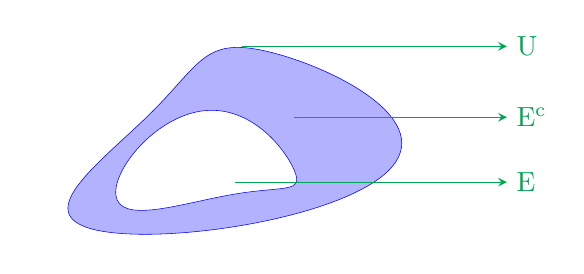
\begin{tikzpicture}[scale=1.5]
            \definecolor{Green}{HTML}{00a652}
            \begin{scope}
                \draw[very thin, fill=Blue!30, draw=Blue] %
                    plot [smooth cycle, tension=1] %
                    coordinates {(1.5, 2.5) (4, 3) (3, 4) (2, 3.5)};       
            \end{scope}
            \begin{scope}[shift={(1.2, 1.5)}]
                \draw[very thin, fill=white, draw=Blue] %
                    plot [smooth cycle, tension=1] % 
                        coordinates {(0.5, 1.25) (1.5, 1.3) (2, 1.5) (1.2, 2)};
            \end{scope}
            \begin{scope}[shift={(2, 3)}]
                \draw[->, >=stealth, Green] (0.7, -0.1)--(3, -0.1)node[right]{$\mathrm{E}$}; 
                \draw[->, >=stealth, Green] (1.2, 0.45)--(3, 0.45)node[right]{$\mathrm{E^c}$}; 
                \draw[->, >=stealth, Green] (0.76, 1.05)--(3, 1.05)node[right]{$\mathrm{U}$}; 
            \end{scope}
        \end{tikzpicture}
        \caption{界点图解}
        \label{界点图解}
    \end{minipage}
\end{figure}

\subsection{上确界存在定理}
% \begin{figure}[!htb]
%     \ctikzfig{Chapter/TikZ//Supremum}
%     \caption{确界直观理解图}
% \end{figure}


我们令 $a_i = a_{{(i-1)}_{10}} = a_{{i}_0}$, $[a_0, a_{10}]$的长度为 $1$,于是可以得到
$a_6 = 0.6 = a_7 - \frac{1}{10},a_7 = 0.7$.把区间放大之后:
区间 $[a_{6_0}, a_{6_{10}}]$的长度为 $\frac{1}{10}$, 于是可以得到
$a_{6_6} = a_{6_7} - \frac{1}{10^3} = a_6 + 7\cdot\frac{1}{10^2}-\frac{1}{10^3}, a_{6_7} = 0.67$.\
然后一直这样迭代下去,根据实数的十进制表示方法可以知道这样的 $\sup\mathrm{E}$是存在且唯一的。

\begin{figure}[!htb]
    \begin{tikzpicture}
        \centering
        \begin{scope}[>=stealth, scale=0.8]
            \foreach \i in {0, 1, ..., 10}
            {
                \draw[ ->] (-0.2, 0)--(10.5, 0);
                \draw[cyan] (6+\i/10, 0)--(6+\i/10, 3pt);
                \draw[red] (6.4, 0)--(6.4, 3pt);
                \draw[thick] (\i, 0)node[below]{$a_{\i}$}--(\i, 3pt);
                \draw[cyan] (6.5, 0) circle [radius=1.02];
                \draw[->, red] (5, 0.2) -- (6.4, 0.2);
            }
        \end{scope}
        \draw[->] (5.12, 0)--(5.12, -2.4)--(6, -2.4);
        % 5.12 = 6.4*0.8,   2.4 = 3*0.8
        \node[below] (A) at (5.12, -1.2) {把这个小区间放大10倍};
        \node[left] (B) at (4, 0.2) {$\sup\mathrm{E}$};
        \begin{scope}[>=stealth, scale=0.8, shift={(8, -3)}]
            \foreach \i in {0, 1, ..., 10}
            {
                \draw[ ->] (-0.2, 0)--(10.5, 0);
                \draw[cyan] (6+\i/10, 0)--(6+\i/10, 3pt);
                \draw[red] (6.4, 0)--(6.4, 3pt);
                \draw[thick] (\i, 0)node[below]{$a_{6_{\i}}$}--(\i, 3pt);
                \draw[cyan] (6.5, 0) circle [radius=1.02];
                \draw[->, red] (5, 0.2) -- (6.4, 0.2);
            }
        \end{scope}
        \node[left] (C) at (10.4, -2.24) {$\sup\mathrm{E}$};
        % 10.4 = (5+8)*0.8,  2.24 = (3-0.2)*0.8
    \end{tikzpicture}
    \caption{确界直观理解图}
\end{figure}

\subsection{内闭一致收敛}
我们都知道函数列一致收敛的几何意义:就是当$n$充分大后的函数曲线系能够都落在关于
极限函数的一个带形区域内(宽为$2\varepsilon$)。
现在你要检查某个区间上函数列是否一致收敛,形象地讲,
闭区间的端点就是你要考虑的范围、限度,
出了这个界你就不考虑这个界以外的曲线能否落在你所预设好的带形区域内。那么,
假设你已经知道在闭区间I上的某个函数列是内闭一致收敛的,
并且很恰巧地你注意到n必须要非常非常大比如$n=1000$,你的这个函数列的曲线系
才开始勉强落入带形区域。
(这种极端情况正是接下来内闭一致收敛不是一致收敛的重要原因。)然后,
你把闭区间$I$向外扩充一点点变成一个开区间$D$,于是,
完全可能出现这样一种情况:$n=1000$已经不能让函数曲线们落入带形区间里了,
你把$n$不断扩大,可是不管$n$怎么大,
开区间的端点附近的$x$点总能找出一部分能让你的曲线系落到带形区间外,
而且你没法定死最无法使你的曲线系落入带形区间的x点以便你能找到最大的$n$,
因为这是开区间!端点处附近永远存在一部分点当你自以为找到足够大的$n$后让
你的曲线系落到带形区间外。
这就是某些内闭一致收敛不一定一致收敛例子的几何解释


\begin{figure}[!htb]
    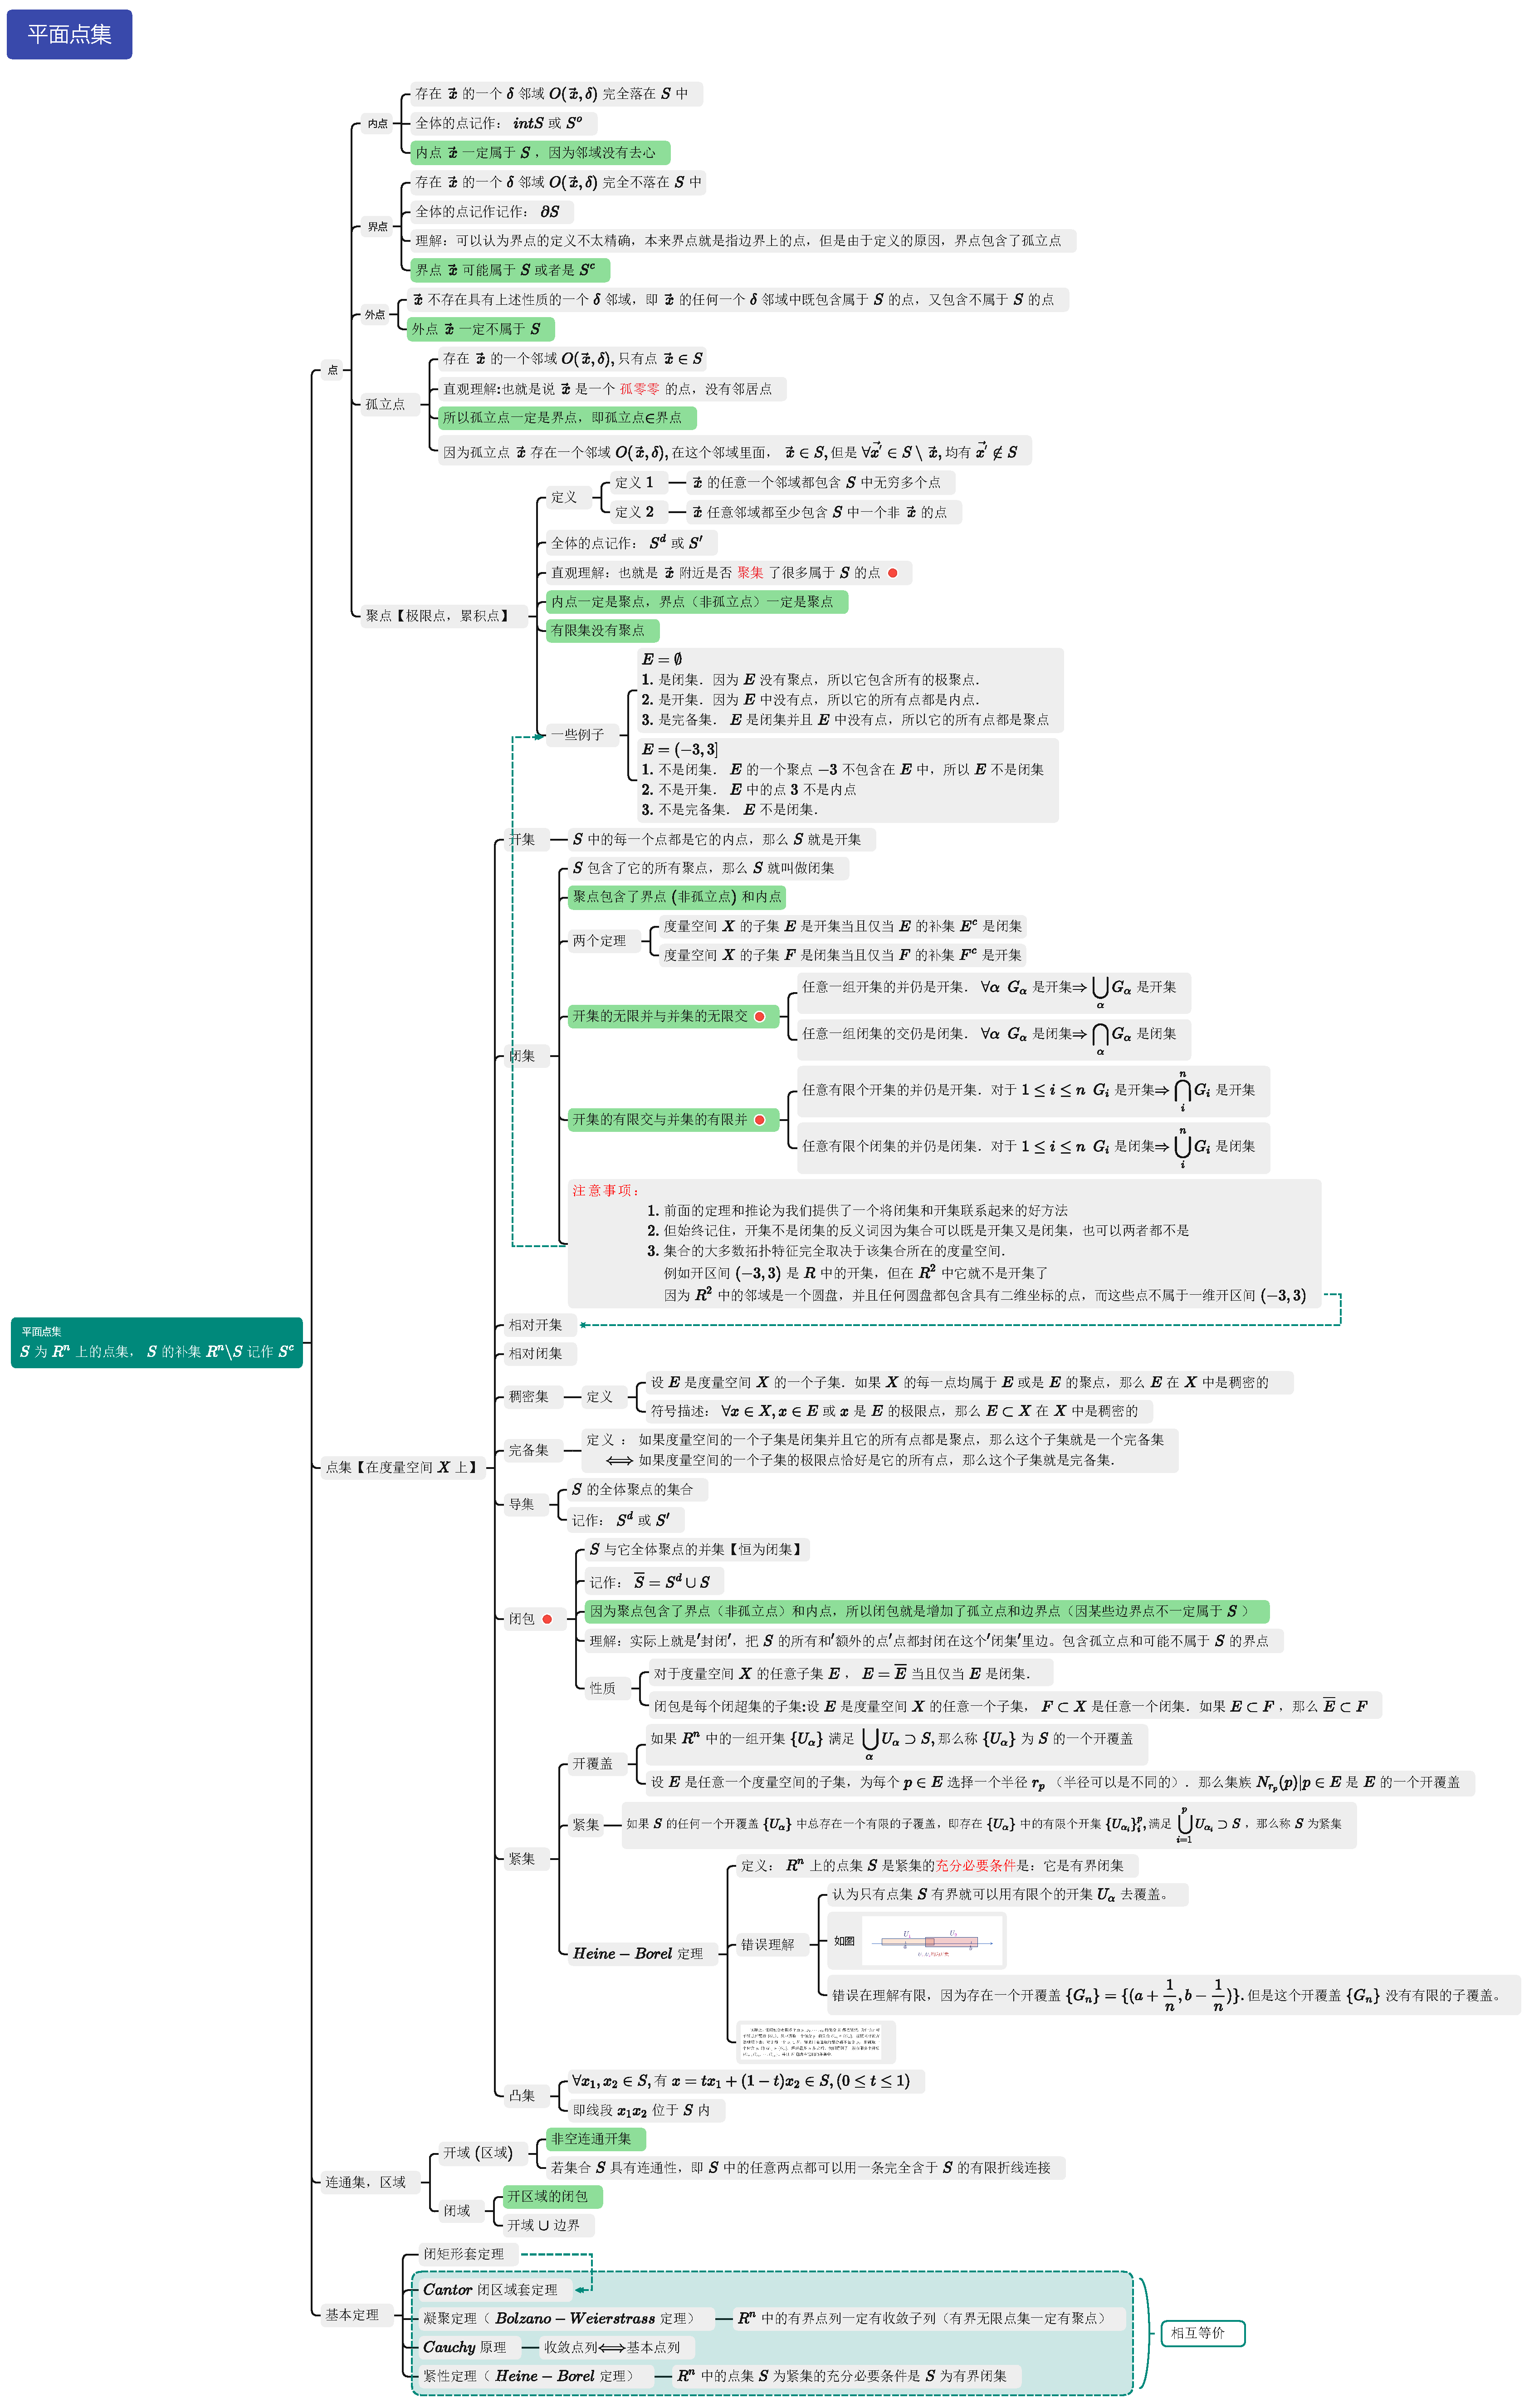
\includegraphics[scale=0.3]{Chapter/TikZ/平面点集.pdf}
    \label{平面点集}
    \caption{平面点集}
\end{figure}